\documentclass[conference]{IEEEtran}
\IEEEoverridecommandlockouts
% The preceding line is only needed to identify funding in the first footnote. If that is unneeded, please comment it out.
\usepackage{cite}
\usepackage{listings}
\usepackage{amsmath,amssymb,amsfonts}
%\usepackage{algorithmic}
\usepackage{amssymb}% http://ctan.org/pkg/amssymb
\usepackage[ruled,linesnumbered]
{algorithm2e}
\usepackage{algpseudocode}
\usepackage{graphicx}
\usepackage{textcomp}
\usepackage{hyperref}
\usepackage{xcolor}
\usepackage[table]{xcolor}
\usepackage{balance}
\usepackage{multirow}
\usepackage{booktabs}
\usepackage{makecell}
\usepackage{balance}
\usepackage{array}
\usepackage{booktabs}
\usepackage{graphicx}
\usepackage{lscape}
\usepackage{longtable}
\usepackage{pifont}% http://ctan.org/pkg/pifont
\newcommand{\cmark}{\ding{51}}%
\newcommand{\xmark}{\ding{55}}%

%\DeclareUnicodeCharacter{2713}{\ding{51}} % ✓
%\DeclareUnicodeCharacter{2717}{\ding{55}} % ✗

\def\BibTeX{{\rm B\kern-.05em{\sc i\kern-.025em b}\kern-.08em
    T\kern-.1667em\lower.7ex\hbox{E}\kern-.125emX}}
\hypersetup{
  colorlinks=true,
  linkcolor=blue,
  citecolor=blue,
  urlcolor=blue
}

\begin{document}

\title{%PPO-Purechain: Adaptive CO$_2$ Transport Scheduling with Verifiable Carbon-Credit Lifecycle Management
PPO-Purechain: Reinforcement-Learning-Based Adaptive CO$_2$ Transport Scheduling with Auditable Blockchain Carbon-Credit Records
}

\author{\IEEEauthorblockN{Ihunanya Udodiri Ajakwe\href{https://orcid.org/0009-0004-9922-2320}{
\includegraphics[scale=0.075]{images/ORCID.png}}, Victor Ikenna Kanu\href{https://orcid.org/0009-0005-5606-8105}{
\includegraphics[scale=0.075]{images/ORCID.png}}, Simeon Okechukwu Ajakwe*\href{https://orcid.org/0000-0002-6973-530X}{
\includegraphics[scale=0.075]{images/ORCID.png}}, Dong-Seong Kim\href{https://orcid.org/0000-0002-2977-5964}{
\includegraphics[scale=0.075]{images/ORCID.png}}}
\IEEEauthorblockA{\textit{Department of IT Convergence Engineering, Kumoh National Institute of Technology, Gumi, Goseong, South Korea} \\
*\textrm{Smart Computing Department, Kyungdong University, Global Campus, South Korea} \\
%\textit{Kumoh National Institute of Technology} 
%Gumi, South Korea \\
{(ihunanya.ajakwe, kanuxavier, simeonajlove)@gmail.com, dskim}@kumoh.ac.kr}
}

\maketitle

\begin{abstract}
Reliable CO$_2$ transportation is essential for large-scale carbon capture, utilization, and storage, yet existing approaches often treat operational optimization and carbon-credit verification as separate problems. This paper
presents PPO--Purechain, an integrated framework that combines adaptive CO$_2$ transport scheduling with permissioned blockchain-based lifecycle
verification. A Proximal Policy Optimization (PPO) agent selects source, sink, route, and batch decisions under normal, high-demand, and energy-spike
conditions, while Purechain records stakeholder registration, validated batch execution, carbon-credit minting, and credit verification. Experiments conducted with synthetically generated transport data show that the trained policy improves reward by 40.3--45.4\% over a fixed heuristic and increases weekly throughput from approximately 17,300 to 32,900 tonnes, corresponding to an 89.9\% gain. The blockchain layer achieves a mean confirmation latency of 1.71~s, a median of 1.67~s, and a 100\% success rate across 78 evaluated transactions. These findings demonstrate the feasibility of connecting adaptive transport control with auditable batch-to-credit traceability in a unified CCUS workflow.
\end{abstract}


\begin{IEEEkeywords}
blockchain, carbon credits, smart contracts, CO$_2$ transportation, compressor scheduling, optimization, PPO, reinforcement learning 
\end{IEEEkeywords}

\vspace{-0.4cm}
\section{\textbf{introduction}}
\label{sec:introduction}

\vspace{-0.3cm}
Carbon capture, utilization, and storage (CCUS) is an important pathway for reducing emissions from industries in which direct electrification remains
difficult. Its large-scale deployment requires reliable transportation of captured carbon dioxide (CO$_2$) from distributed sources to utilization or
geological storage sites. Such networks must coordinate source availability, sink capacity, route conditions, energy use, and operational constraints while maintaining high throughput and traceable transport records.

Existing studies mainly address strategic source--sink matching, pipeline routing, capacity allocation, and cost minimization
~\cite{zhang2022advances,velasco2024optimizing}. Agent-based modeling and deep-learning approaches have improved multimodal network analysis and pipeline monitoring~\cite{uddin2025agent,kim2024real}, but they do not learn adaptive batch-scheduling policies from operational feedback~\cite{ajakwe2026predblock}. Reinforcement learning has
shown potential for dynamic carbon and industrial-process control ~\cite{schulman2017ppo,li2024integrating,raven2024machine}; however, its integration with verifiable CO$_2$ transport and carbon-credit operations
remains limited.

Blockchain-based carbon systems provide traceability, distributed trust, and automated verification~\cite{muzumdar2022permissioned,
suta2023systematic,luo2024carbon}. Nevertheless, most existing solutions record carbon information after the operational activity has occurred and do not maintain a direct association among an adaptive scheduling decision, the executed transport batch, participating stakeholders, and the resulting credit.

This paper proposes a PPO--Purechain framework that combines adaptive CO$_2$ transport scheduling with permissioned blockchain verification. The main
contributions are:

\begin{itemize}
    \item An integrated architecture linking PPO-generated transport decisions
    to tamper-evident batch and carbon-credit records;

    \item A PPO scheduler evaluated under normal, high-demand, and energy-spike
    scenarios against a fixed heuristic baseline; and

    \item A Purechain smart-contract workflow supporting stakeholder
    registration, batch scheduling, credit minting, and credit verification.
\end{itemize}

\vspace{-0.3cm}
\section{\textbf{methodology and system architecture}}
\label{sec:methodology}

\vspace{-0.2cm}
\subsection{System Model}

\vspace{-0.2cm}
As shown in Fig.~\ref{fig:system_architecture}, the proposed framework comprises a transport simulation environment, a PPO agent, an execution and validation
interface, and the Purechain blockchain layer. The environment provides CO$_2$ availability, sink demand, route capacity, energy conditions, and active batch status. PPO selects the source, sink, route, and batch quantity, while validated outputs are transferred to Purechain for immutable recording and credit processing. Optimization and verification are intentionally separated. PPO performs the computationally intensive scheduling off-chain, whereas Purechain verifies and records the resulting transport and credit lifecycle. This separation limits on-chain computation while retaining traceability from the scheduling decision to the corresponding credit record.

\begin{figure}
\centerline{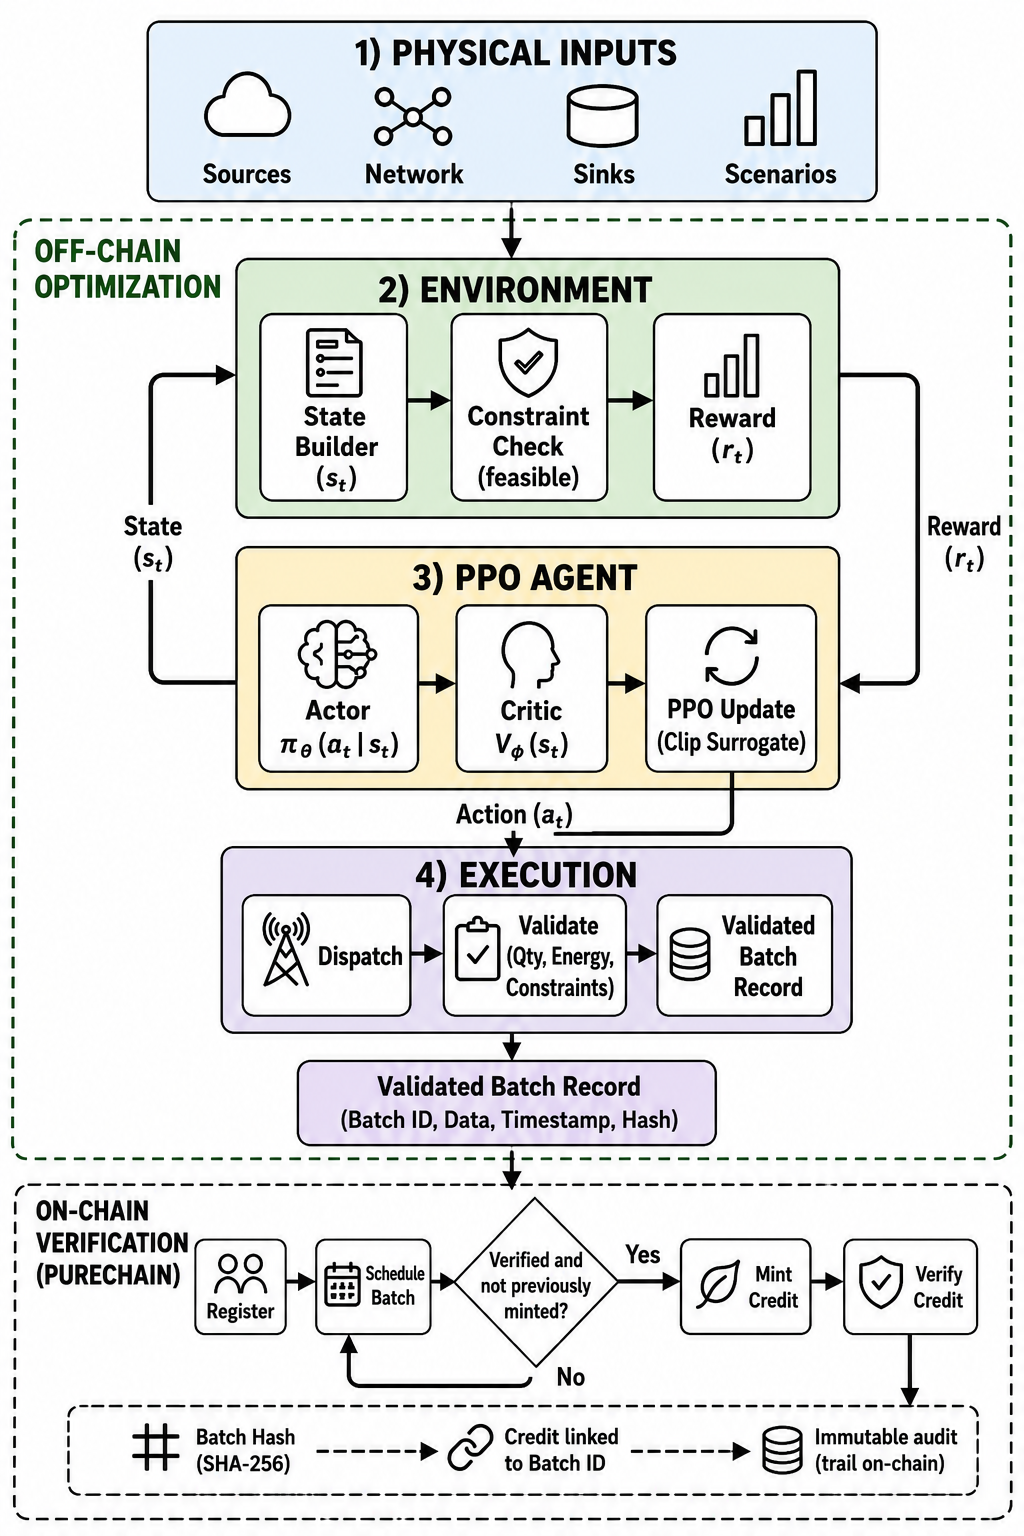
\includegraphics[width=0.50\textwidth]{images/system_design2.png}}
\vspace{-0.5cm}
\caption{Layered system architecture of the proposed PPO--Purechain framework for adaptive CO$_2$ transport scheduling and blockchain-based carbon-credit verification.}
\label{fig:system_architecture}
\end{figure}

\subsection{Transport Environment and PPO Scheduler}

The CO$_2$ transport process is modeled as a discrete-time Markov Decision Process
$\mathcal{M}=\langle\mathcal{S},\mathcal{A},P,R,\gamma\rangle$.
Each episode represents one operational week with 168 hourly decision steps. The state is expressed as:

\vspace{-0.3cm}
\begin{equation}
s_t =
\left[
q_t^{\mathrm{src}},
d_t^{\mathrm{sink}},
c_t^{\mathrm{route}},
e_t,
b_t,
\tau_t
\right],
\label{eq:state}
\end{equation}

where the variables denote source availability, sink demand or capacity, route conditions, energy state, active batches, and time, respectively. An action
$a_t$ specifies the selected source, sink, route, and transported quantity. Actions violating source, sink, or route constraints are rejected or penalized.

The PPO reward balances delivered CO$_2$ against energy use, infeasible actions, and simulated leakage:

\vspace{-0.4cm}
\begin{equation}
r_t =
w_q\widetilde{Q}_t
-w_e\widetilde{E}_t
-w_vV_t
-w_lL_t,
\label{eq:reward}
\end{equation}

\vspace{-0.3cm}
where $\widetilde{Q}_t$ and $\widetilde{E}_t$ are normalized throughput and energy terms, while $V_t$ and $L_t$ penalize constraint violations and simulated leakage events. Accordingly, the evaluation measures avoidance of simulated
violations rather than physical leakage prevention in an operational pipeline. PPO updates the actor policy using the clipped surrogate objective
~\cite{schulman2017ppo}:

\vspace{-0.5cm}
\begin{equation}
L^{\mathrm{CLIP}}(\theta)=
\mathbb{E}_{t}
\left[
\min
\left(
\rho_t(\theta)\hat{A}_t,
\operatorname{clip}
\left(
\rho_t(\theta),1-\epsilon,1+\epsilon
\right)\hat{A}_t
\right)
\right],
\label{eq:ppo}
\end{equation}


\vspace{-0.1cm}
where
$\rho_t(\theta)=
\pi_{\theta}(a_t|s_t)/
\pi_{\theta_{\mathrm{old}}}(a_t|s_t)$,
$\hat{A}_t$ is the estimated advantage, and $\epsilon$ limits excessive policy updates. 
%%%%PPO hyperparameter configuration
\textcolor{black}{The action space is discretized as at = [src, sink, route, q], where src/sink/route are selected from $|$S$|$=6 sources, $|$K$|$=4 sinks, and $|$R$|$=8 candidate routes, and $q \in \{0, 50, 100, \dots, 500\}$ tonnes is the batch quantity in 50-tonne increments, giving a discrete action space of size 6×4×8×11 = 2,112. Table I summarizes the PPO training configuration.}


\textcolor{black}{A fixed rule-based heuristic is used as the baseline, and both methods are evaluated under identical environment configurations}. 

%\textcolor{blue}{Two baselines are used for comparison. The first is a nearest-feasible heuristic: at each decision step it selects the source–sink pair with the largest current available quantity subject to route-capacity and energy constraints, without accounting for future demand or energy variability. The second is a greedy-throughput heuristic that maximizes immediate delivered CO$_2$ per step regardless of downstream energy cost, providing an upper-bound-seeking but myopic comparison. Both baselines use identical environment configurations and constraint checks as the PPO agent, isolating the effect of learned adaptivity from rule-based decision-making.}

\vspace{-0.5cm}
\begin{table}[!htbp]
\tiny
\caption{PPO hyperparameters}
\vspace{-0.3cm}
\label{tab:ppo_hyperparams}
\centering
\begin{tabular}{@{}ll@{}}
\toprule
\textbf{Parameter} & \textbf{Value} \\
\midrule
Policy/value network      & 2-layer MLP, 128 units \\
Learning rate             & $3 \times 10^{-4}$ \\
Clip range ($\epsilon$)   & 0.2 \\
Discount factor ($\gamma$) & 0.99 \\
GAE $\lambda$             & 0.95 \\
Batch size                & 64 \\
Epochs per update         & 10 \\
Training episodes         & 590 \\
N Steps per Rollout       & 2,048 \\
Episode length          & 168 steps \\
Entropy Coefficient & 0.01 \\
Value Function Coefficient & 0.5 \\
Total Timesteps & 100,000 \\
%Data split    & 70\%/15\%/15\% \\
\bottomrule
\end{tabular}
\end{table}


\vspace{-0.5cm}
\subsection{Purechain Verification}

\vspace{-0.2cm}
Purechain is a permissioned blockchain that records validated scheduler outputs and manages the carbon-credit lifecycle~\cite{ajakwe2025ebctc}. Its smart contracts perform stakeholder registration, batch scheduling, credit minting, and credit verification. For each validated batch $b$, the system stores:

\vspace{-0.4cm}
\begin{equation}
H_b =
\operatorname{SHA256}
\left(
ID_b \Vert ID_s \Vert ID_k \Vert Q_b \Vert E_b \Vert t_b
\right),
\label{eq:hash}
\end{equation}

\vspace{-0.2cm}
where the fields represent the batch, source, sink, transported quantity, energy record, and timestamp. A credit is minted only when the batch exists, satisfies the validation conditions, and has not previously been credited. The credit is linked to its originating batch identifier, while larger operational data remain off-chain to reduce storage overhead.

\subsection{Integrated Operational Workflow}
\label{subsec:integrated_workflow}

The transport environment generates the current system state, which the trained PPO policy evaluates to select the source, destination, route, and batch quantity; the environment then checks operational constraints and returns throughput, energy cost, feasibility status, and learning feedback. Each feasible decision is converted into a structured batch record and submitted to Purechain, where smart contracts manage batch scheduling, transport validation, carbon-credit minting, and verification of the batch digest, stakeholder identities, credit identifier, and transaction status. Thus, PPO provides adaptive control through environmental feedback, while Purechain preserves end-to-end traceability across registration, scheduling, minting, and verification.


\subsection{Experimental Configuration and Metrics}
\label{subsec:experimental_setup}

The experiments use synthetically generated data representing CO$_2$ source availability, sink demand, route capacity, energy conditions, and transport-batch status under normal, high-demand, and energy-spike scenarios. Consequently, the
reported results demonstrate performance within the configured simulation environment rather than a deployed CO$_2$ transport network.

The PPO policy is trained using weekly episodes of 168 hourly steps. The agent was configured for 100,000 timesteps and completed 590 full weekly episodes, corresponding to 99,120 environment steps. Training performance is evaluated using mean reward, reward variability, and weekly CO$_2$ throughput, while the fixed policy is tested under the three operating scenarios and compared with the heuristic baseline. The percentage improvement over the heuristic baseline is calculated as:

\vspace{-0.3cm}
\begin{equation}
I =
\frac{M_{\mathrm{PPO}}-M_{\mathrm{base}}}
{\left|M_{\mathrm{base}}\right|}
\times 100\%,
\label{eq:performance_improvement}
\end{equation}

\vspace{-0.2cm}
where $M_{\mathrm{PPO}}$ and $M_{\mathrm{base}}$ denote the PPO and baseline values for the evaluated reward or throughput metric.

The blockchain layer is evaluated using transaction confirmation latency and transaction success rate. Confirmation latency is measured as the elapsed time
between transaction submission and confirmed inclusion in the blockchain. Success rate is defined as the proportion of submitted transactions that are successfully confirmed. The evaluation covers stakeholder registration, batch scheduling, credit minting, and credit verification. An additional stakeholder-registration stress test is conducted to examine whether transaction completion and latency remain stable under an increased number of consecutive requests.


\section{\textbf{results and discussion}}
\label{sec:results}

The proposed framework was evaluated from two complementary perspectives: (i) the learning and operational performance of the Proximal Policy Optimization (PPO) agent, and (ii) the execution efficiency and reliability of the Purechain blockchain network. The evaluation focused on convergence behavior, robustness under different operating conditions, CO$_2$ transport throughput, transaction latency, and transaction success rate.

\subsection{PPO Training Convergence}
\label{subsec:ppo_convergence}
\begin{figure}
\centerline{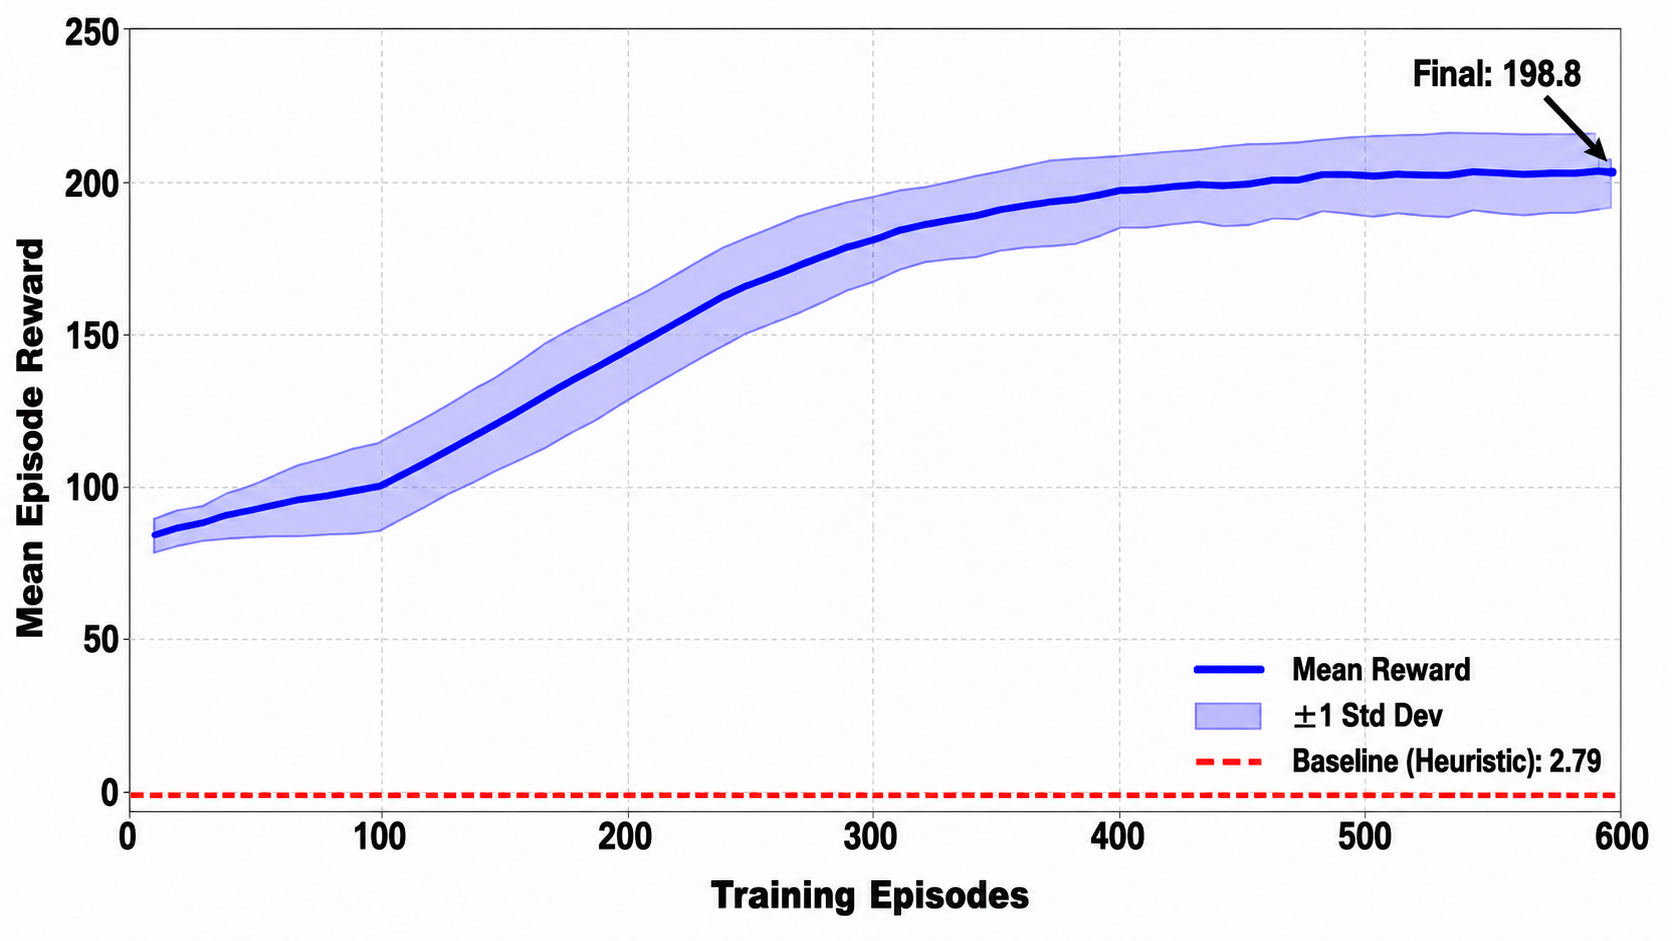
\includegraphics[width=0.46\textwidth]
{images/Training_curve2}}
\vspace{-0.5cm}
\caption{PPO agent training progress showing the increase in mean episode reward and the corresponding standard-deviation interval.}
\label{ppo_training}
\end{figure}

Fig.~\ref{ppo_training} presents the mean episode reward obtained during PPO training. The reward increased from approximately 94 in the initial episodes to a final value of 198.8. Most of the performance improvement occurred within the first 400 episodes, after which the curve gradually approached a stable plateau near 200.



The increasing reward indicates that the agent progressively learned a more effective scheduling policy from its interaction with the simulated CO$_2$ transport environment. The relatively small fluctuations observed during the later training stage suggest that the policy had largely converged and was no longer undergoing substantial behavioral changes. In addition, the bounded standard-deviation region shows that the final policy maintained comparatively consistent performance across repeated evaluations.

These results demonstrate that PPO was able to learn a stable decision policy within the available training horizon. Although small variations remained near convergence, no major reward collapse or unstable oscillation was observed. This is important for CO$_2$ transport scheduling, where abrupt policy changes could produce inconsistent routing, batching, or energy-allocation decisions.

\vspace{-0.2cm}
\subsection{Performance Under Different Operating Scenarios}
\label{subsec:scenario_performance}

\vspace{-0.1cm}
To assess whether the learned policy could operate beyond a single nominal condition, the PPO agent was compared with the heuristic baseline under normal-demand, high-demand, and energy-spike scenarios. As shown in Fig.~\ref{scenario_comparison}, the PPO agent achieved mean rewards of 212.1, 206.7, and 213.7 under the three scenarios, respectively. In comparison, the heuristic method obtained corresponding rewards of 147.8, 147.3, and 147.0. The PPO agent therefore improved the mean reward by approximately 43.5\% under normal conditions, 40.3\% under high demand, and 45.4\% during the energy-spike scenario. The consistent improvement across all scenarios indicates that the learned policy was not restricted to a single operating pattern. In particular, the agent maintained a reward above 200 even when the system experienced increased demand or abnormal energy conditions.

\begin{figure}
\centerline{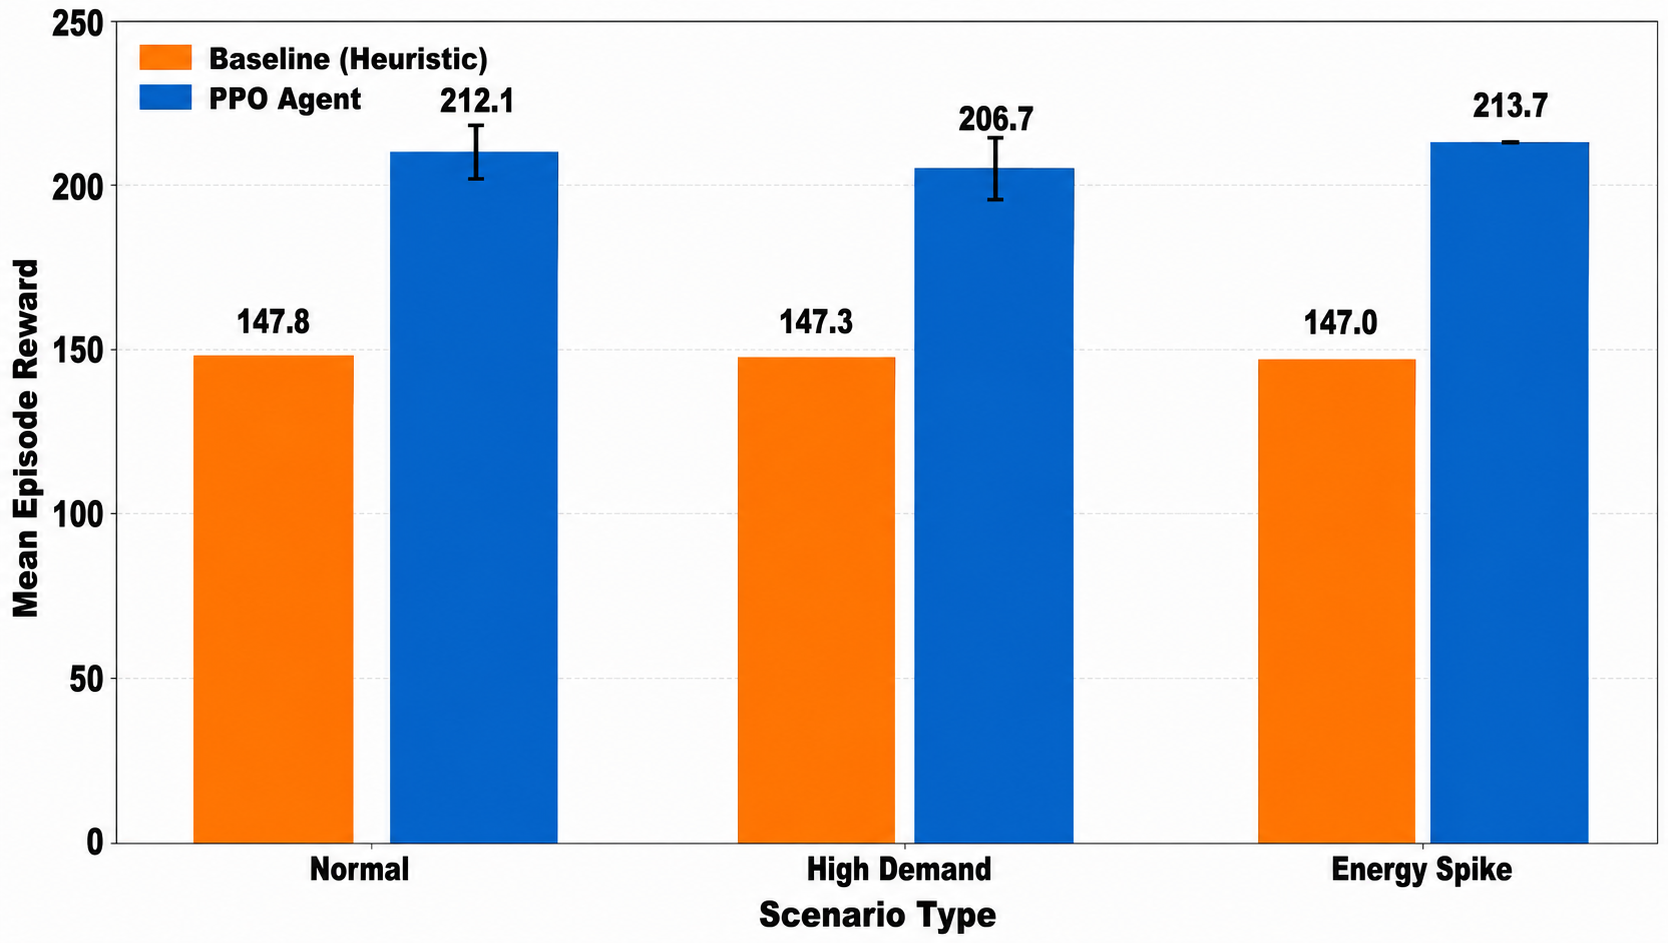
\includegraphics[width=0.52\textwidth]{images/fig3_scenario_comparison2.png}}
\vspace{-0.5cm}
\caption{Mean episode reward of the heuristic baseline and PPO agent under different scenarios (normal, high-demand, and energy-spike)}
\label{scenario_comparison}
\end{figure}

The slightly lower PPO reward under the high-demand scenario suggests that transport congestion or resource limitations made the scheduling problem more difficult. Nevertheless, the agent still substantially outperformed the heuristic scheduler. The highest reward was observed during the energy-spike scenario, indicating that the PPO agent was able to exploit changes in energy availability more effectively than the fixed-rule baseline. Overall, the learned policy adapts its scheduling decisions to changing operating conditions more effectively than static heuristics constrained by predetermined rules.

\vspace{-0.2cm}
\subsection{CO$_2$ Throughput Improvement}
\vspace{-0.1cm}
Fig.~\ref{fig:throughput} shows that weekly CO$_2$ throughput increased from approximately 17,300 to 32,900 tonnes/week, corresponding to an 89.9\%
improvement. The largest gains occurred during the middle training stage before the curve approached a plateau, indicating that PPO progressively removed
inefficient scheduling decisions and approached the effective capacity of the simulated network.

\vspace{-0.5cm}
\begin{figure}[!htbp]
    \centering
    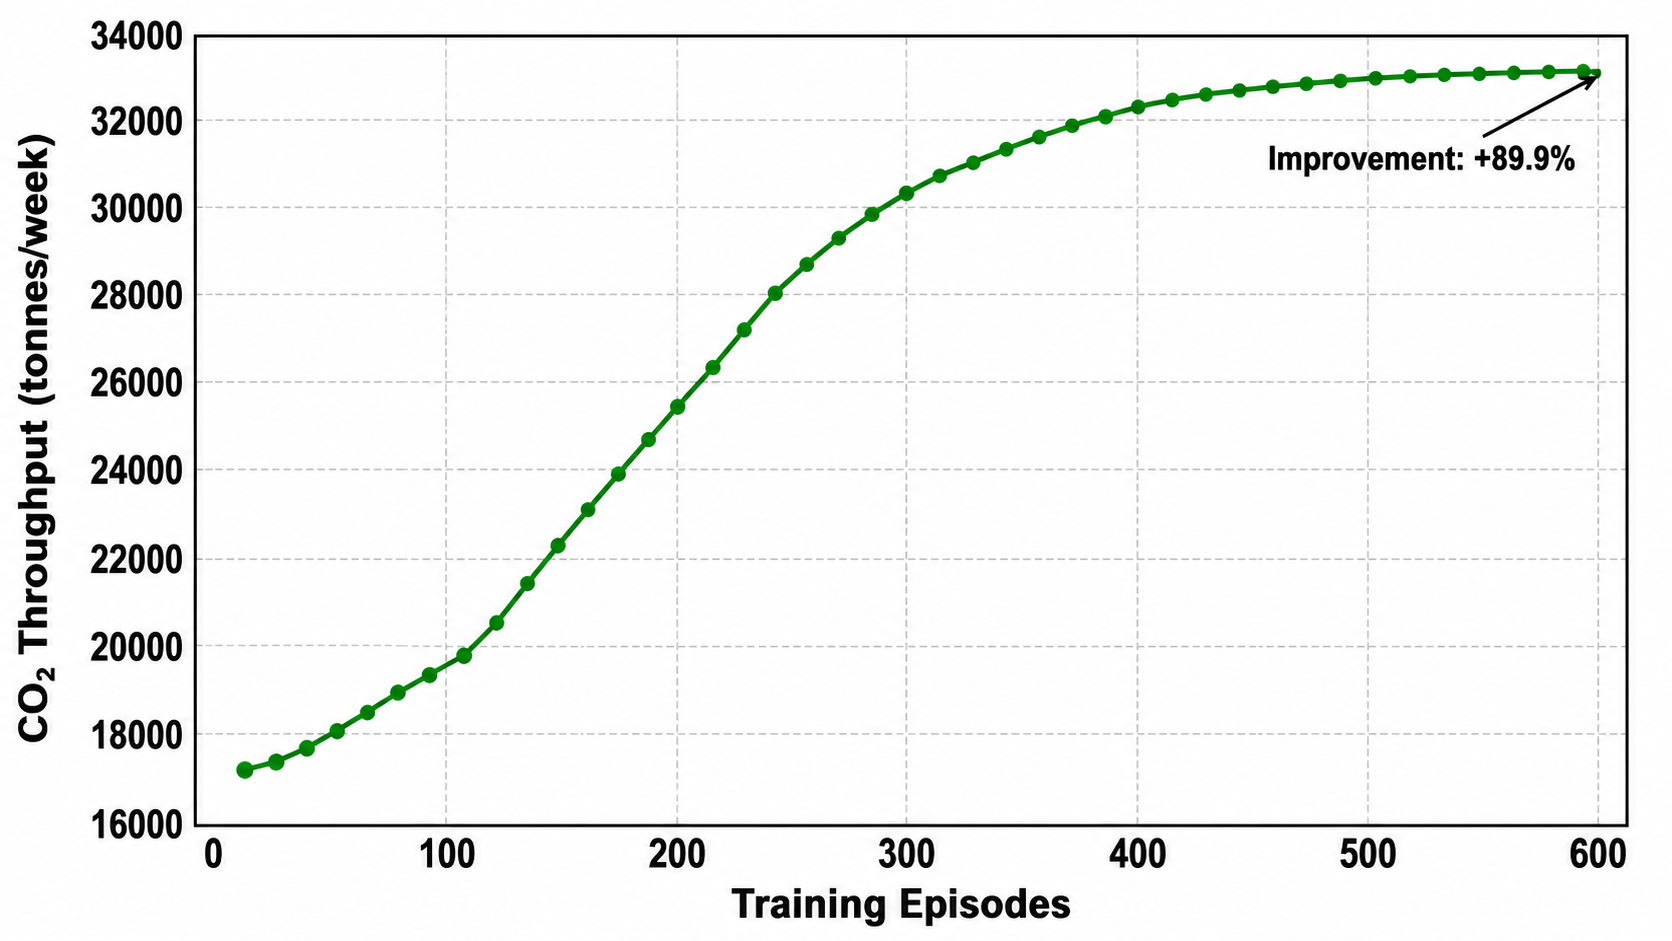
\includegraphics[width=\columnwidth]
    {images/throughput_Progress2.png}
    \vspace{-0.5cm}
    \caption{CO$_2$ transport throughput progression during PPO training.}
    \label{fig:throughput}
\end{figure}

\vspace{-0.5cm}
\subsection{Blockchain Performance}

\vspace{-0.2cm}
Fig.~\ref{fig:blockchain}(a) shows that Purechain achieved mean and median confirmation latencies of 1.71~s and 1.67~s, respectively. Credit minting
exhibited the greatest variation because it required additional validation and state updates, whereas scheduling and verification generally completed more quickly. The initial test included 38 transactions, followed by 40 stress-test registrations. As shown in Fig.~\ref{fig:blockchain}(b), all 78 transactions
were confirmed successfully, and the stress-test mean latency remained close to the overall value at 1.72~s. These results indicate reliable execution under the tested workload, although larger concurrent and fault-injection experiments are
needed to establish production-scale performance.

 \vspace{-0.3cm}
\begin{figure}[!htbp]
    \centering
    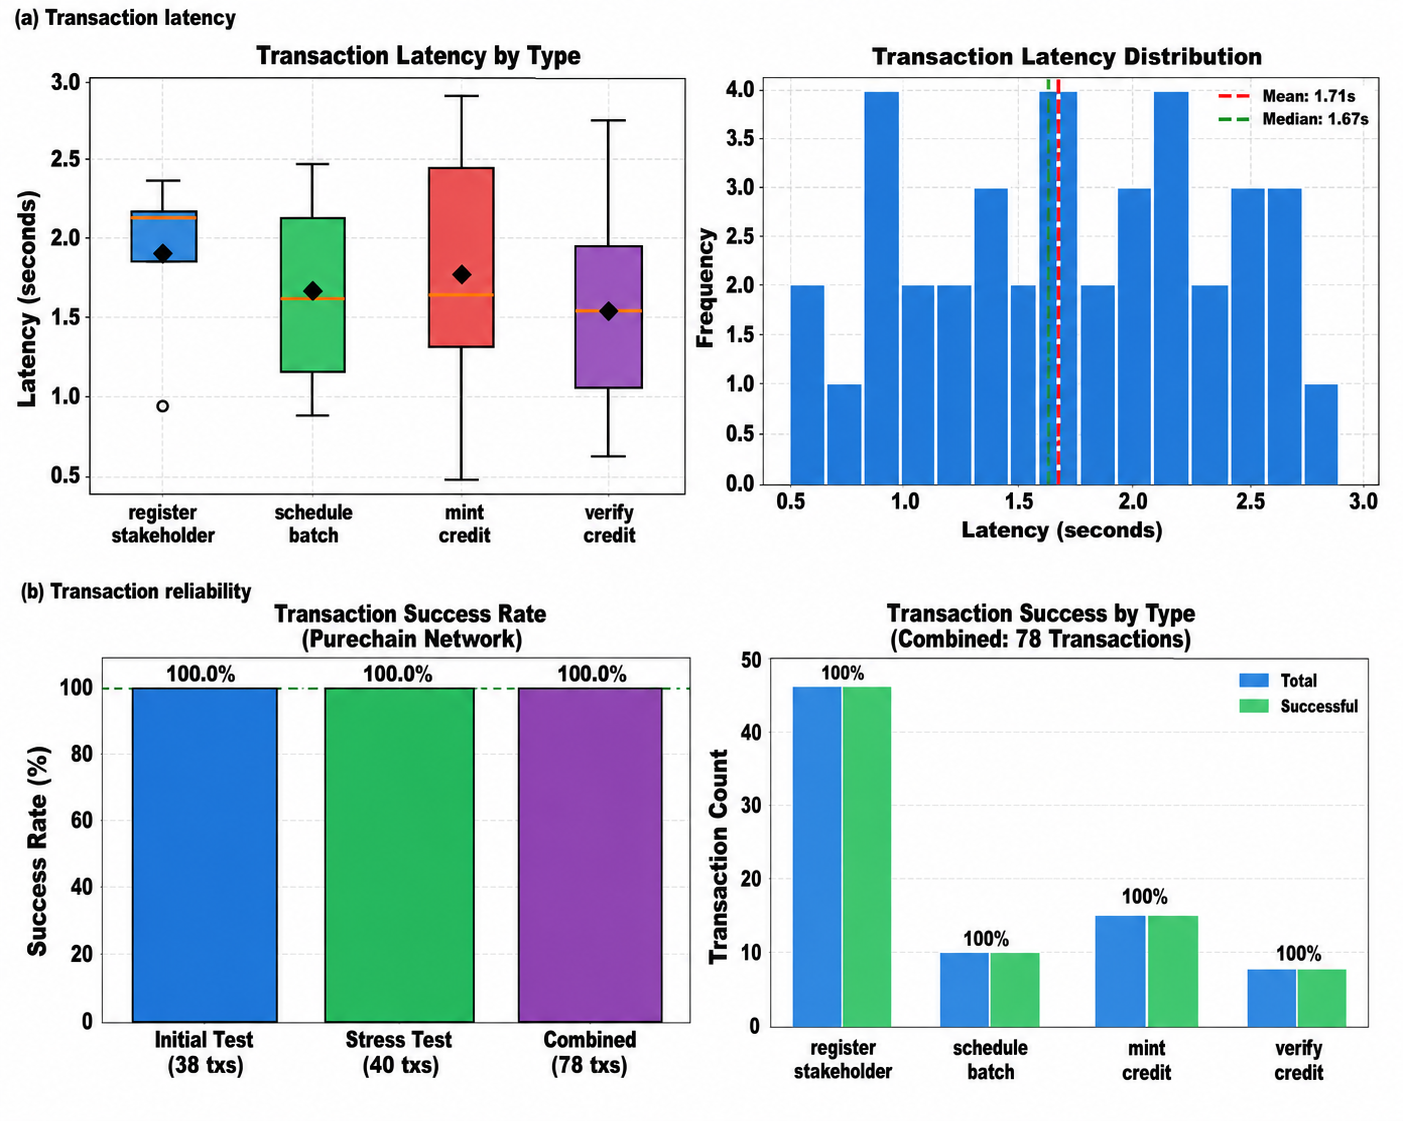
\includegraphics[width=\columnwidth]
    {images/Block_Lat_Rel2.png}
    \vspace{-0.5cm}
    \caption{Purechain performance: (a) transaction latency and distribution;
    and (b) success rate under initial and stress-test workloads.}
    \label{fig:blockchain}
\end{figure}

\vspace{-0.3cm}
\section{\textbf{conclusion}}
\label{sec:conclusion}
\vspace{-0.2cm}
This paper presented PPO--Purechain, an integrated framework for adaptive CO$_2$ transport scheduling and auditable carbon-credit lifecycle management.
The PPO agent consistently outperformed the heuristic baseline across normal, high-demand, and energy-spike scenarios, improving mean reward by
40.3--45.4\% and increasing weekly throughput by 89.9\%. Purechain further provided batch-level traceability with a mean transaction latency of 1.71~s and successful confirmation of all 78 evaluated transactions, linking stakeholder
registration, scheduling, credit minting, and verification within one permissioned workflow. Since the current results were obtained using synthetic transport data and a limited blockchain workload, and rely on a comparison against a single fixed heuristic baseline, they demonstrate feasibility within the configured simulation rather than field-level deployment. Future work will validate the framework using real transport and energy data, stronger optimization and reinforcement-learning baselines, larger source--sink networks, and concurrent blockchain workloads under validator and network-failure conditions.



\vspace{-0.2cm}
\section*{\textbf{acknowledgment}}
\fontsize{9}{3}\selectfont
%\vspace{-0.15cm}
This work was partly supported by the IITP grant funded by the Korea government (MSIT) (IITP-2026-RS-2020-II201612, 25\%), Priority Research Center Program through the NRF funded by the MEST (2018R1A6A1A03024003, 25\%), MSIT, Korea, under the ITRC support program (IITP-2026-RS-2024-00438430, 25\%), and NRF funded by the Ministry of Education (RS-2025-25431637, 25\%).
\balance
\vspace{-0.27cm}
\bibliographystyle{IEEEtran}
\bibliography{newref,Bibliography}

\end{document}

